\documentclass{article}
    \title{Tarea 2}
    \author{Miguel Torres Eric Giovanni}
    \usepackage[spanish,activeacute]{babel}
    \usepackage{mathtools}
    \usepackage{graphicx}
    \usepackage{anysize}
    \usepackage{multicol}
    \usepackage{amsmath}
    \usepackage{amssymb}
    \graphicspath{{images/}}

    \marginsize{1.5cm}{3cm}{3cm}{3cm}
    
    \begin{document}
        \maketitle

        1. Suponga que un experimento consiste en escoger un 
        número al azar dentro del intervalo {0,1}. Para cada 
        resultado $w$ del experimento se expresa a este 
        número en su expansión decimal $w=0.a_{1}a_{2}a_{3}...$ 
        en donde $a_{i}\in\{0,1,...,9\}, i=1,2,...$ Para cada una de las 
        siguientes variables aleatorias determine si ésta es discreta 
        o continua y en cualquier caso el conjunto de valores que 
        puede tomar: \vspace{.1cm}

        a)$X(w)=a_{1}$\vspace{.1cm}

        \hspace{.7cm} Es discreta y los valores qu puede tomar son $(.1,.2,...,.9)$\vspace{.1cm}

        b)$Y(w)=0.0a_{1}a_{2}a_{3}...$\vspace{.1cm}

        \hspace{.7cm} Es continua y los valores que puede tomar están en el intervalo $(0,0.1)$\vspace{.3cm}

        2. Comprueba que las siguientes funciones son de 
        probabilidad:\vspace{.1cm}

        a) $f(x) = \left \{ 
            \begin{matrix}
                \frac{x-1}{2^{x}}$\hspace{1cm} si $x = 1,2,... \\ $
                $0$ \hspace{1cm} $e.o.c$
            $\end{matrix}
        \right .$\vspace{.1cm}

        \framebox{Solución}\vspace{.1cm}

        i) $f(x) > 0$ cumple porque $x=1,2,...$ vale $\frac{x-1}{2^x}$\vspace{.1cm}

        ii) $\displaystyle\int_{\infty}^{\infty}f(x) = 1$\vspace{.1cm}

        $\Rightarrow \displaystyle\int_{1}^{\infty}f(x)dx 
        = \displaystyle\int_{1}^{\infty}\frac{x-1}{2^x}dx$, integrando por partes: \vspace{.1cm}
        
        
        $= \frac{x-1}{ln(2)(2^x)}-\displaystyle\int_{1}^{\infty}\frac{-1}{ln(2)(2^x)}dx =
        $

        b) $f(x) = \left \{ 
            \begin{matrix}
                \frac{(1-p)p^{x-1}}{1-p^n}$\hspace{1cm} si $x=1,...,n (0<p<1)\\ $ constante
                $0$ \hspace{1cm} $e.o.c$
            $\end{matrix}
        \right .$\vspace{.1cm}

        \framebox{Solución}\vspace{.1cm}

        i) $f(x) > 0$, ocurre pues $x = 1,..., n$ esta vale: $\frac{(1-p)p^{x-1}}{1-p^n}$\vspace{.1cm}

        ii) $\displaystyle\sum_{1}^{n}\frac{(1-p)p^{x-1}}{1-p^n} = 1$\vspace{.1cm}

        $\therefore $ es función de probabilidad\vspace{.1cm}

        c) $f(x) = \left \{ 
            \begin{matrix}
                \frac{\frac{1}{2}}{\sqrt{x}}$\hspace{1cm} si $0 < x < 1 \\ $
                $0$ \hspace{1cm}$e.o.c$
            $\end{matrix}
        \right .$\vspace{.1cm}

        \framebox{Solución}\vspace{.1cm}

        i) $f(x) > 0$\vspace{.1cm}

        ii) $\displaystyle\int_{0}^{1}\frac{\frac{1}{2}}{\sqrt{x}}dx = 
        \frac{1}{2}\displaystyle\int_{0}^{1}x^{\frac{-1}{2}} 
        = \frac{1}{2}(\frac{x^{\frac{1}{2}}}{1/2})  = x^{\frac{1}{2}} = 
        \left . \sqrt{x} \right |_{0}^{1} = 1$\vspace{.1cm}

        $\therefore $ es función de probabilidad

        d) $f(x) = \left \{ 
            \begin{matrix}
                \frac{3(1-|x|)^2}{2}$\hspace{1cm} si $-1 < x < 1 \\ $
                $0$ \hspace{1cm} $e.o.c$
            $\end{matrix}
        \right .$\vspace{.1cm}

        \framebox{Solución}\vspace{.1cm}

        i) $f(x) > 0$\vspace{.1cm}

        ii) $\displaystyle\int_{0}^{1}f(x)dx = \displaystyle\int_{0}^{1}\frac{3(1-|x|)^2}{2}dx
        = \frac{3}{2} \displaystyle\int_{0}^{1}(1-|x|)^2$, integrando por cambio de variable \vspace{.1cm}

        $\Rightarrow \frac{-3}{2}\displaystyle\int_{0}^{1}u^2du = 
        \frac{-3}{2}(\left . \frac{u^3}{3} \right |_{0}^{1}) = 
        (- \left . \frac{(1-|x|)^3}{3} \right |_{0}^{1}) = \frac{1}{3}$\vspace{.1cm}

        $\therefore $ Por lo que no es función de probabilidad

        3. Determina si la función $f(x)$ puede ser una función de 
        densidad. En caso afirmativo, encuentra el valor de la 
        constante c.\vspace{.1cm}

        $f(x) = \left \{ 
                \begin{matrix}
                    c(2x-x^3)$\hspace{1cm} si $0 < x < 2 \\ $
                    $0$ \hspace{1cm} $e.o.c$
                $\end{matrix}
            \right .$\vspace{.1cm}

        $\displaystyle\int_{0}^{2}c(2x-x^3) dx=1$\vspace{.1cm}

        $\Rightarrow c\displaystyle\int_{0}^{2}2x-x^3 dx=c[(x^2|_0^2)-(\frac{x^4}{4}|_0^2)]=c[4-\frac{16}{4}]=c[4-4] \Rightarrow c=1$\vspace{.1cm}

            $f(x) = \left \{ 
                \begin{matrix}
                    c(2x-x^2)$\hspace{1cm} si $0 < x < 2 \\ $
                    $0$ \hspace{1cm} $e.o.c$
                $\end{matrix}
            \right .$\vspace{.1cm}

            $\displaystyle\int_{0}^{2}c(2x-x^2) dx=1$\vspace{.1cm}

            $\Rightarrow c\displaystyle\int_{0}^{2}2x-x^2 dx=c[(x^2|_0^2)-(\frac{x^3}{3}|_0^2)]=c[4-\frac{8}{3}]=\frac{4}{3}c \Rightarrow c = \frac{3}{4}$\vspace{.3cm}

        4. Una moneda equilibrada se lanza repetidamente hasta 
        obtener un mismo resultado por tercera ocasión, no 
        necesariamente de manera consecutiva. Encuentra la función 
        de probabilidad de la variable aleatoria que registra el número 
        de lanzamientos necesarios hasta obtener el resultado 
        mencionado.\vspace{.1cm}

        $S_x={3,4,5}$, $\mathbb{P}(aguila) = \frac{1}{2}$, $\mathbb{P}(sol) =
         \frac{1}{2}$\vspace{.1cm}

         $f(x) = \left \{ 
            \begin{matrix}
                1$\hspace{1cm} con probabilidad $\frac{1}{2}\\ $
                $0$ \hspace{1cm} con probabilidad $\frac{1}{2}$
            $\end{matrix}
        \right .$\vspace{.1cm}

        \framebox{Solución}\vspace{.1cm}
        
        $f(x)=(\frac{1}{2})^x(\frac{1}{2})^{1-x}\mathbb{I}_{0,1}(x)$\vspace{.3cm}

        5. Muestra que la siguiente función es de probabilidad y 
        encuentra la correspondiente función de distribución y 
        grafica ambas funciones.\vspace{.1cm}

        $f(x) = \left \{ 
                \begin{matrix}
                    4e^{-4x}$\hspace{1cm} si $x > 0 \\ $
                    $0$ \hspace{1cm} $e.o.c$
                $\end{matrix}
            \right .$\vspace{.3cm}

            \framebox{Solución:}\vspace{.3cm}

            $(1)$ ¿Es una función de probabilidad?\vspace{.2cm}
    
            \hspace{.5cm} $i)$ $f(x)\geq 0$\vspace{.2cm}
    
            \hspace{.7cm} $f(x)>0$ pues $x>0$
            
            \hspace{.5cm} $ii)$ $\displaystyle{\int_{-\infty}^{\infty}}f(x) dx=1$
    
            \hspace{.7cm} $\displaystyle{\int_{-\infty}^{\infty}}4e^{-4x} dx=\displaystyle{\int_{0}^{\infty}}4e^{-4x}dx$ $u=-4x$, $du=-4dx$\vspace{.2cm}
    
            \hspace{.7cm}  $\Rightarrow \displaystyle\int_{0}^{\infty}e^{u} du = \left . e^{u} \right |_0^\infty= e^\infty - e^0 = 1$\vspace{.3cm}
    
            $\therefore$ $f(x)$ es una función de probabilidad.\vspace{.3cm}
    
            $(2)$ La función de distribución $(F(x))$:\vspace{.2cm}
    
            Como $f(x)=\frac{d}{dx}F(x)$, entonces $F(x)=\int f(x) dx$.\vspace{.2cm}
    
            $\int 4e^{-4x} dx = -e^{-4x} $\vspace{.2cm}
    
            $\therefore F(x)=-e^{-4x}$.\vspace{.3cm}
    
            \begin{center}
                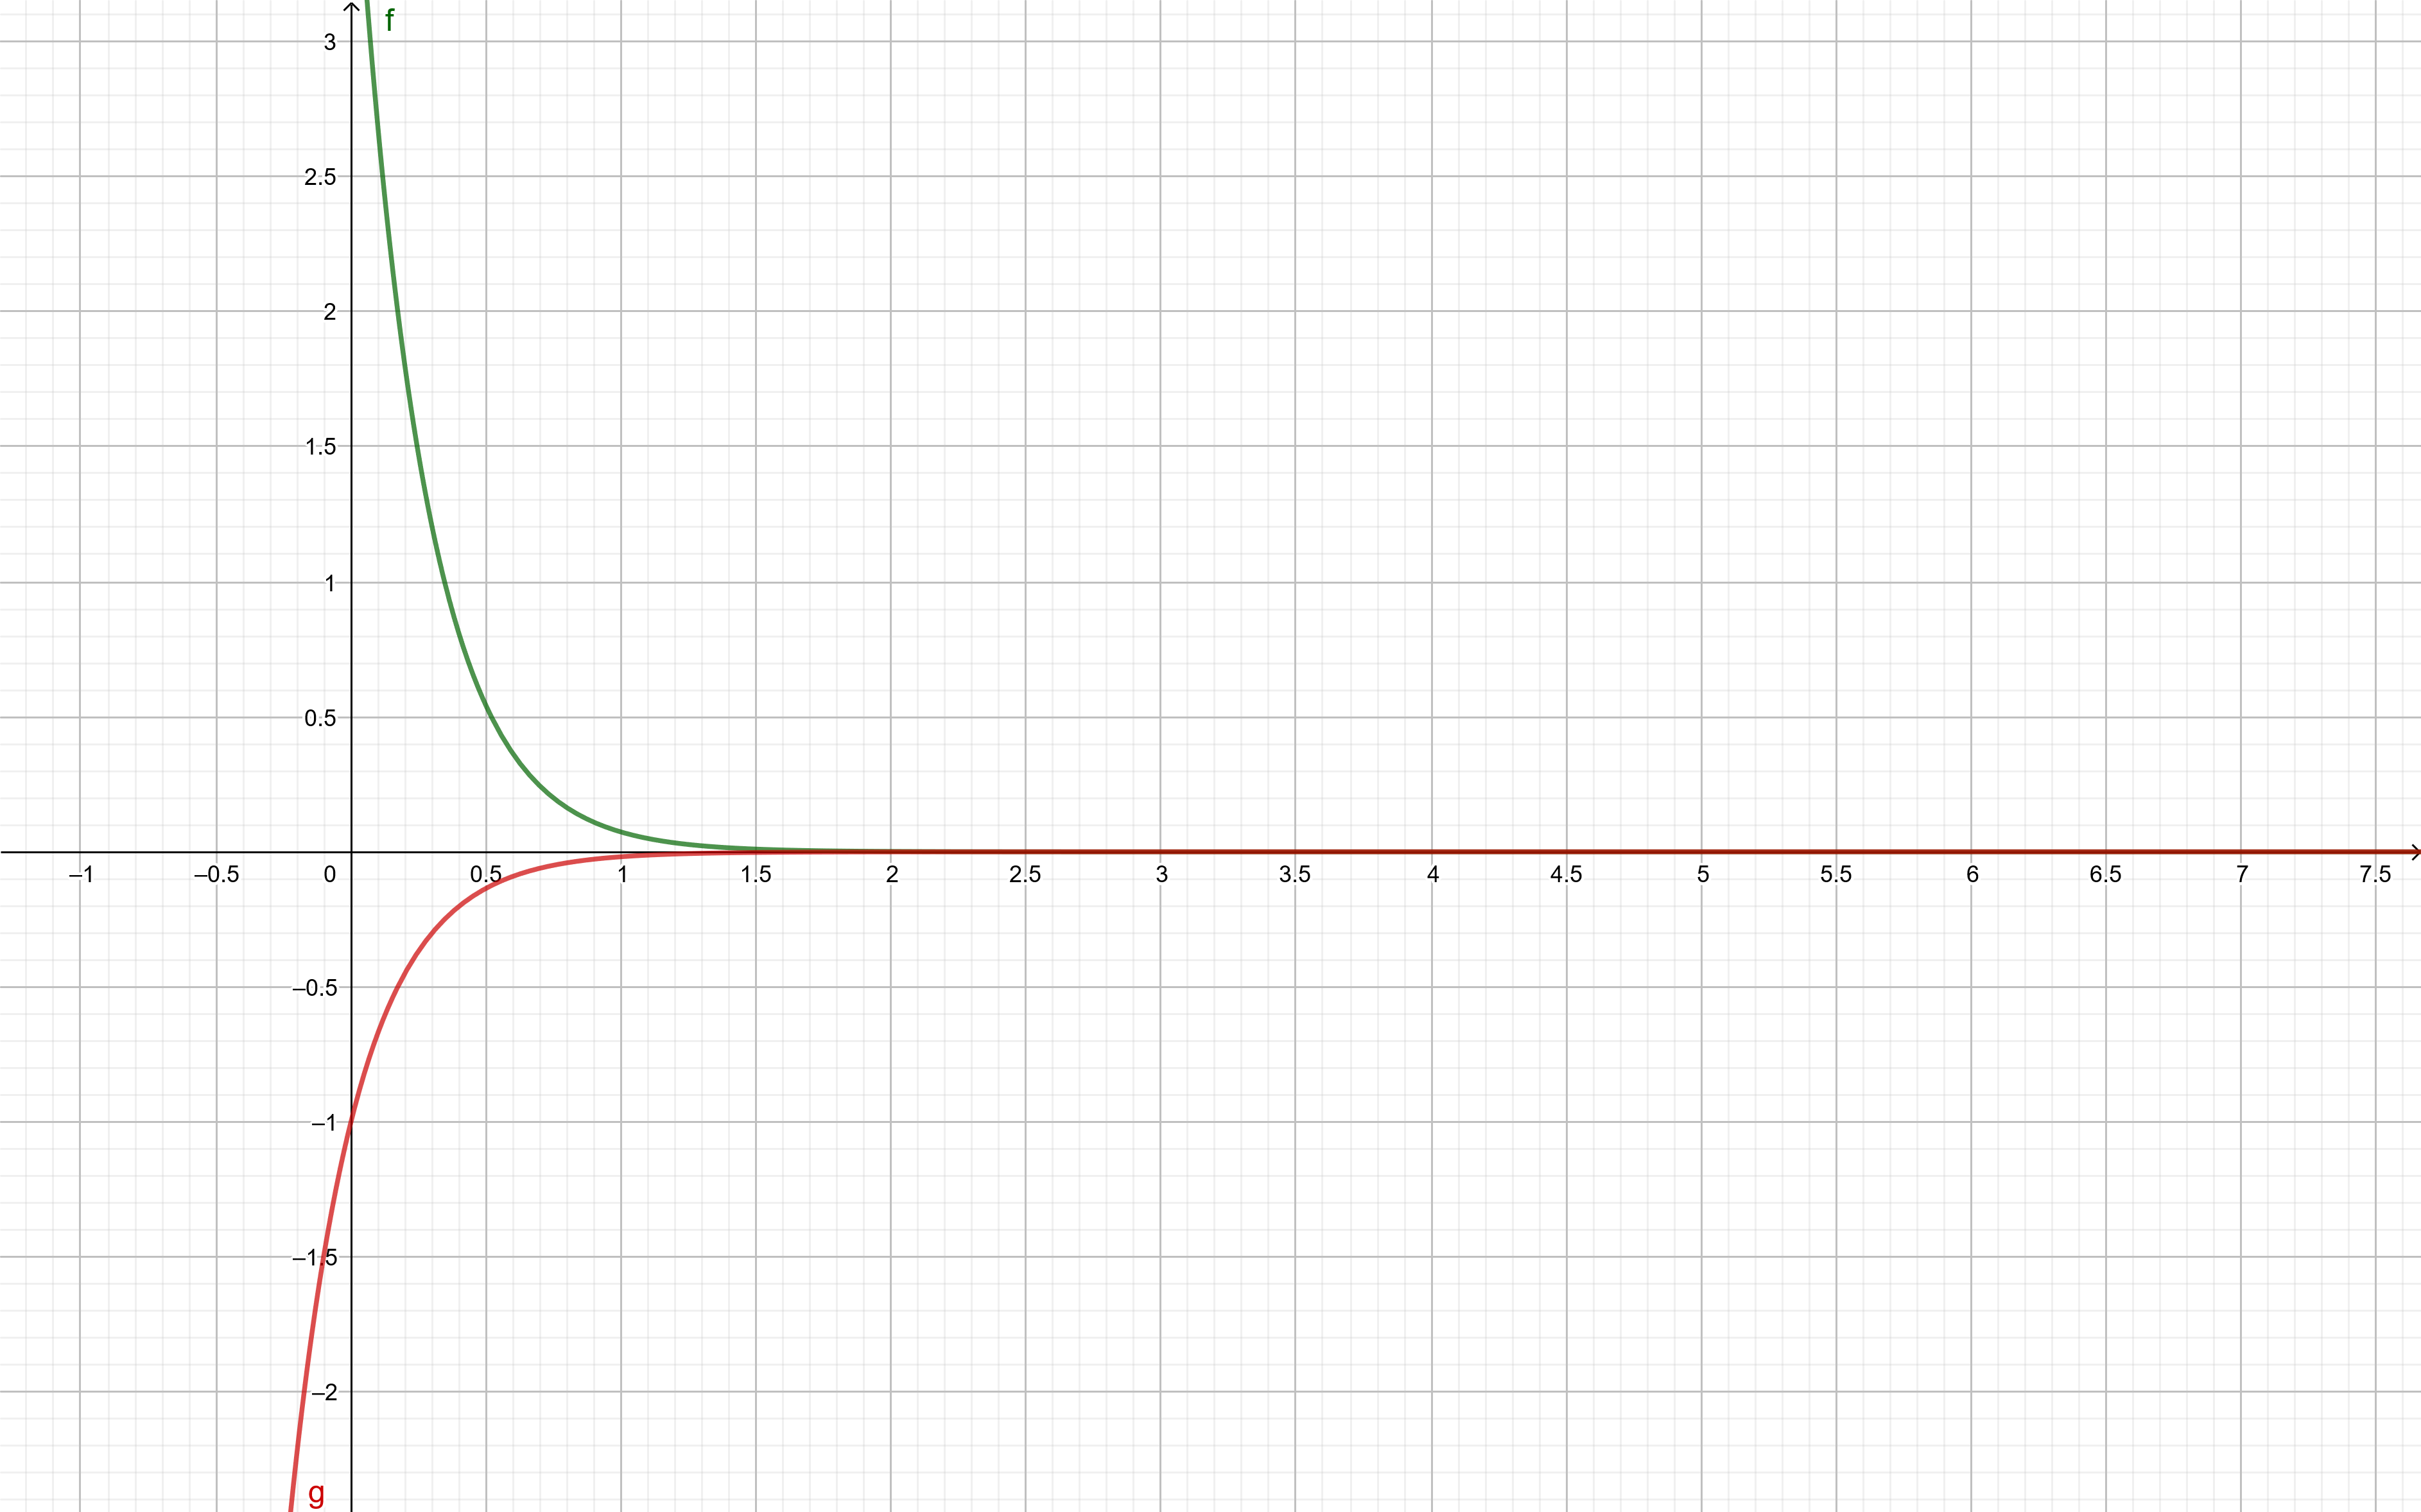
\includegraphics[scale=0.07]{proba.png}   
            \end{center}

        6. Sea $X$ una variable aleatoria continua con función de 
        densidad\vspace{.1cm}

        $f(x) = \left \{ 
                \begin{matrix}
                    \frac{1}{x^2}$\hspace{1cm} si $x \geq 0 \\ $
                    $0$ \hspace{1cm} $e.o.c$
                $\end{matrix}
            \right .$\vspace{.1cm}

        a) Grafica $f(x)$ y comprueba que es funcion de densidad\vspace{.1cm}

        \begin{center}
            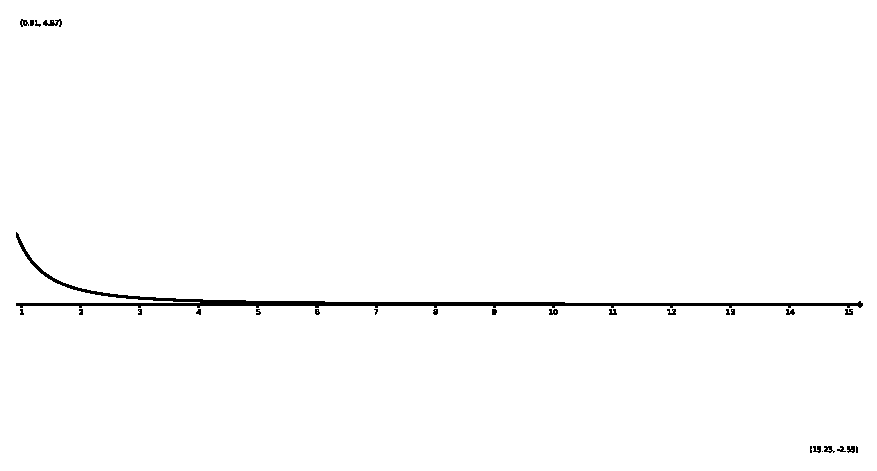
\includegraphics[scale=0.9]{grafica.eps}   
        \end{center}

        b)Encuentra y grafica la funcion de distribución de $X$. \vspace{.1cm}

        c) Encuentra y grafica la funcion de distribución de la variable 
        $Y = e^{-x}$\vspace{.3cm}

        7. Calcula la esperanza de las siguientes variables 
        aleatorias con función de probabilidad: \vspace{.3cm}

        a)$f(x) = \left \{ 
                \begin{matrix}
                    \frac{2x}{n(n+1)}$\hspace{1cm} si $x=1,2,...,n \\ $
                    $0$ \hspace{1cm} $e.o.c$
                $\end{matrix}
            \right .$\vspace{.1cm}

        b)$f(x) = \left \{ 
                \begin{matrix}
                    \frac{x}{4}e^{\frac{x}{2}}$\hspace{1cm} si $x > 2 \\ $
                    $0$ \hspace{1cm} $e.o.c$
                $\end{matrix}
            \right .$\vspace{.3cm}

        8. a) Demuestra las siguientes fórmulas\vspace{.1cm}

        i. Sea $X$ una variable aleatoria discreta con función de 
        distribución $F(X)$, con esperanza finita y posibles 
        valores dentro del conjunto ${0,1,2,...}$, entonces 
        $E(X)=\displaystyle\sum_{x=0}^{\infty}(1-F(x))$\vspace{.1cm}

        \framebox{Demostración:}\vspace{.1cm}

        Sabemos lo siguiente: $F(x)=\mathbb{P}[X\leq x]$ y $1-F(x)=\mathbb{P}[X>x]$, entonces...\vspace{.1cm}

        $\displaystyle\sum_{x=0}^{infty} (1-F(x))=\displaystyle\sum_{x=0}^{\infty} (\displaystyle\sum_{y=x+1}^{\infty} f(y))=\displaystyle\sum_{y=1}^{\infty}{\displaystyle\sum_{x=0}^{y-1}}f(y)
        =\displaystyle\sum_{y=1}^{\infty}yf(y)+0=\displaystyle\sum_{y=0}^{\infty}yf(y)=E(X)$ $\blacksquare$

        ii. Sea $X$ una variable aleatoria continua con función de 
        distribución $F(X)$, con esperanza finita y posibles valores 
        en el intervalo $[0, \infty)$, entonces 
        $E(X)=\displaystyle\int_0^\infty (1-F(x))$\vspace{.1cm}

        \framebox{Demostración:}\vspace{.1cm}

        Sabemos lo siguiente: $F(x)=\displaystyle\int_{-\infty}^{\infty}f(u)du$, entonces...\vspace{.1cm}

        $\displaystyle\int_{0}^{\infty}(1-F(x)) dx=\displaystyle\int_{0}^{\infty}{\displaystyle\int_{x}^{\infty}}f(y)dydx=\displaystyle\int_{0}^{\infty}{\displaystyle\int_{0}^{y}}f(y)dxdy=\displaystyle\int_{0}^{\infty}yf(y)dy=E(X)$ $\blacksquare$

        b)Usando el ejercicio anterior, encuentra la esperanza de $X$ 
        cuando ésta tiene función de distribución: \vspace{.1cm}

        i. $F(x) = \left \{ 
                \begin{matrix}
                    1-(\frac{1}{2})^k$\hspace{1cm} si $k\leq x < k+1; k=1,2,...\\ $
                    $0$ \hspace{1cm} si $x < 1$
                $\end{matrix}
            \right .$\vspace{.1cm}

        ii. $F(x) = \left \{ 
                \begin{matrix}
                    1-e^{-x}$\hspace{1cm} si $x > 0 \\ $
                    $0$ \hspace{1cm} $e.o.c$
                $\end{matrix}
            \right .$\vspace{.3cm}

        9. Demustra o proporciona un contraejemplo: \vspace{.1cm}

        a) Si $E(X)=0$ entonces $X=0$\vspace{.1cm}

        FALSO. Tomemos  $F(x) = \left \{ 
            \begin{matrix}
                \frac{1}{2}$\hspace{1cm} si $x=-1,1 \\ $
                $0$ \hspace{1cm} $e.o.c$
            $\end{matrix}
        \right .$\vspace{.1cm}

        $E(X)= -\frac{1}{2}+\frac{1}{2}=0$\vspace{.3cm}

        b) Si $E(X)=E(Y)$ entonces $X=Y$\vspace{.1cm}

        FALSO. Tomemos dos funciones:\vspace{.1cm}

        $f(x_1) = \left \{ 
                \begin{matrix}
                    2x$\hspace{1cm} si $0 <x< 1 \\ $
                    $0$ \hspace{1cm} $e.o.c$
                $\end{matrix}
            \right .$\vspace{.1cm}

        $E(X_1)=\displaystyle{\int_{-\infty}^{\infty}}xf(x) dx=\displaystyle{\int_{0}^{1}}xf(x) dx=\frac{2x^3}{3}|_0^1=\frac{2}{3}$\vspace{.2cm}

        $f(x_2) = \left \{ 
                \begin{matrix}
                    x$\hspace{1cm} si $0 <x< \displaystyle\sqrt[3]{2} \\ $
                    $0$ \hspace{1cm} $e.o.c$
                $\end{matrix}
            \right .$\vspace{.1cm}

        $E(X_2)=\displaystyle{\int_{-\infty}^{\infty}}xf(x) dx=\displaystyle{\int_{0}^{\displaystyle\sqrt[3]{2}}}x^2 dx=\frac{x^3}{3}|_0^{\sqrt[3]{2}}=\frac{2}{3}$\vspace{.1cm}

        Tenemos que $E(X_1)=E(X_2)$ pero $X_1\neq X_2$\vspace{.3cm}


        10. El ladrón de Bagdad ha sido colocado en una prisión 
        en donde hay tres puertas. Una de las puertas conduce a un 
        túnel que requiere de un día de travesía y que lo regresa a 
        la misma prisión. Otra de las puertas lo conduce a otro túnel, 
        aun más largo, que lo regresa nuevamente a la prisión, pero 
        después de 3 días de recorrido. Finalmente, la tercera puerta 
        lo conduce a la libertad inmediatamente. Suponga que el 
        ladrón escoge al azar cada una de estas puertas, una por una, 
        hasta quedar libre. Encuentre el número promedio de días 
        que le toma al ladrón quedar en libertad.\vspace{.1cm}

        \framebox{Solución:}\vspace{.1cm}

        \begin{center}
            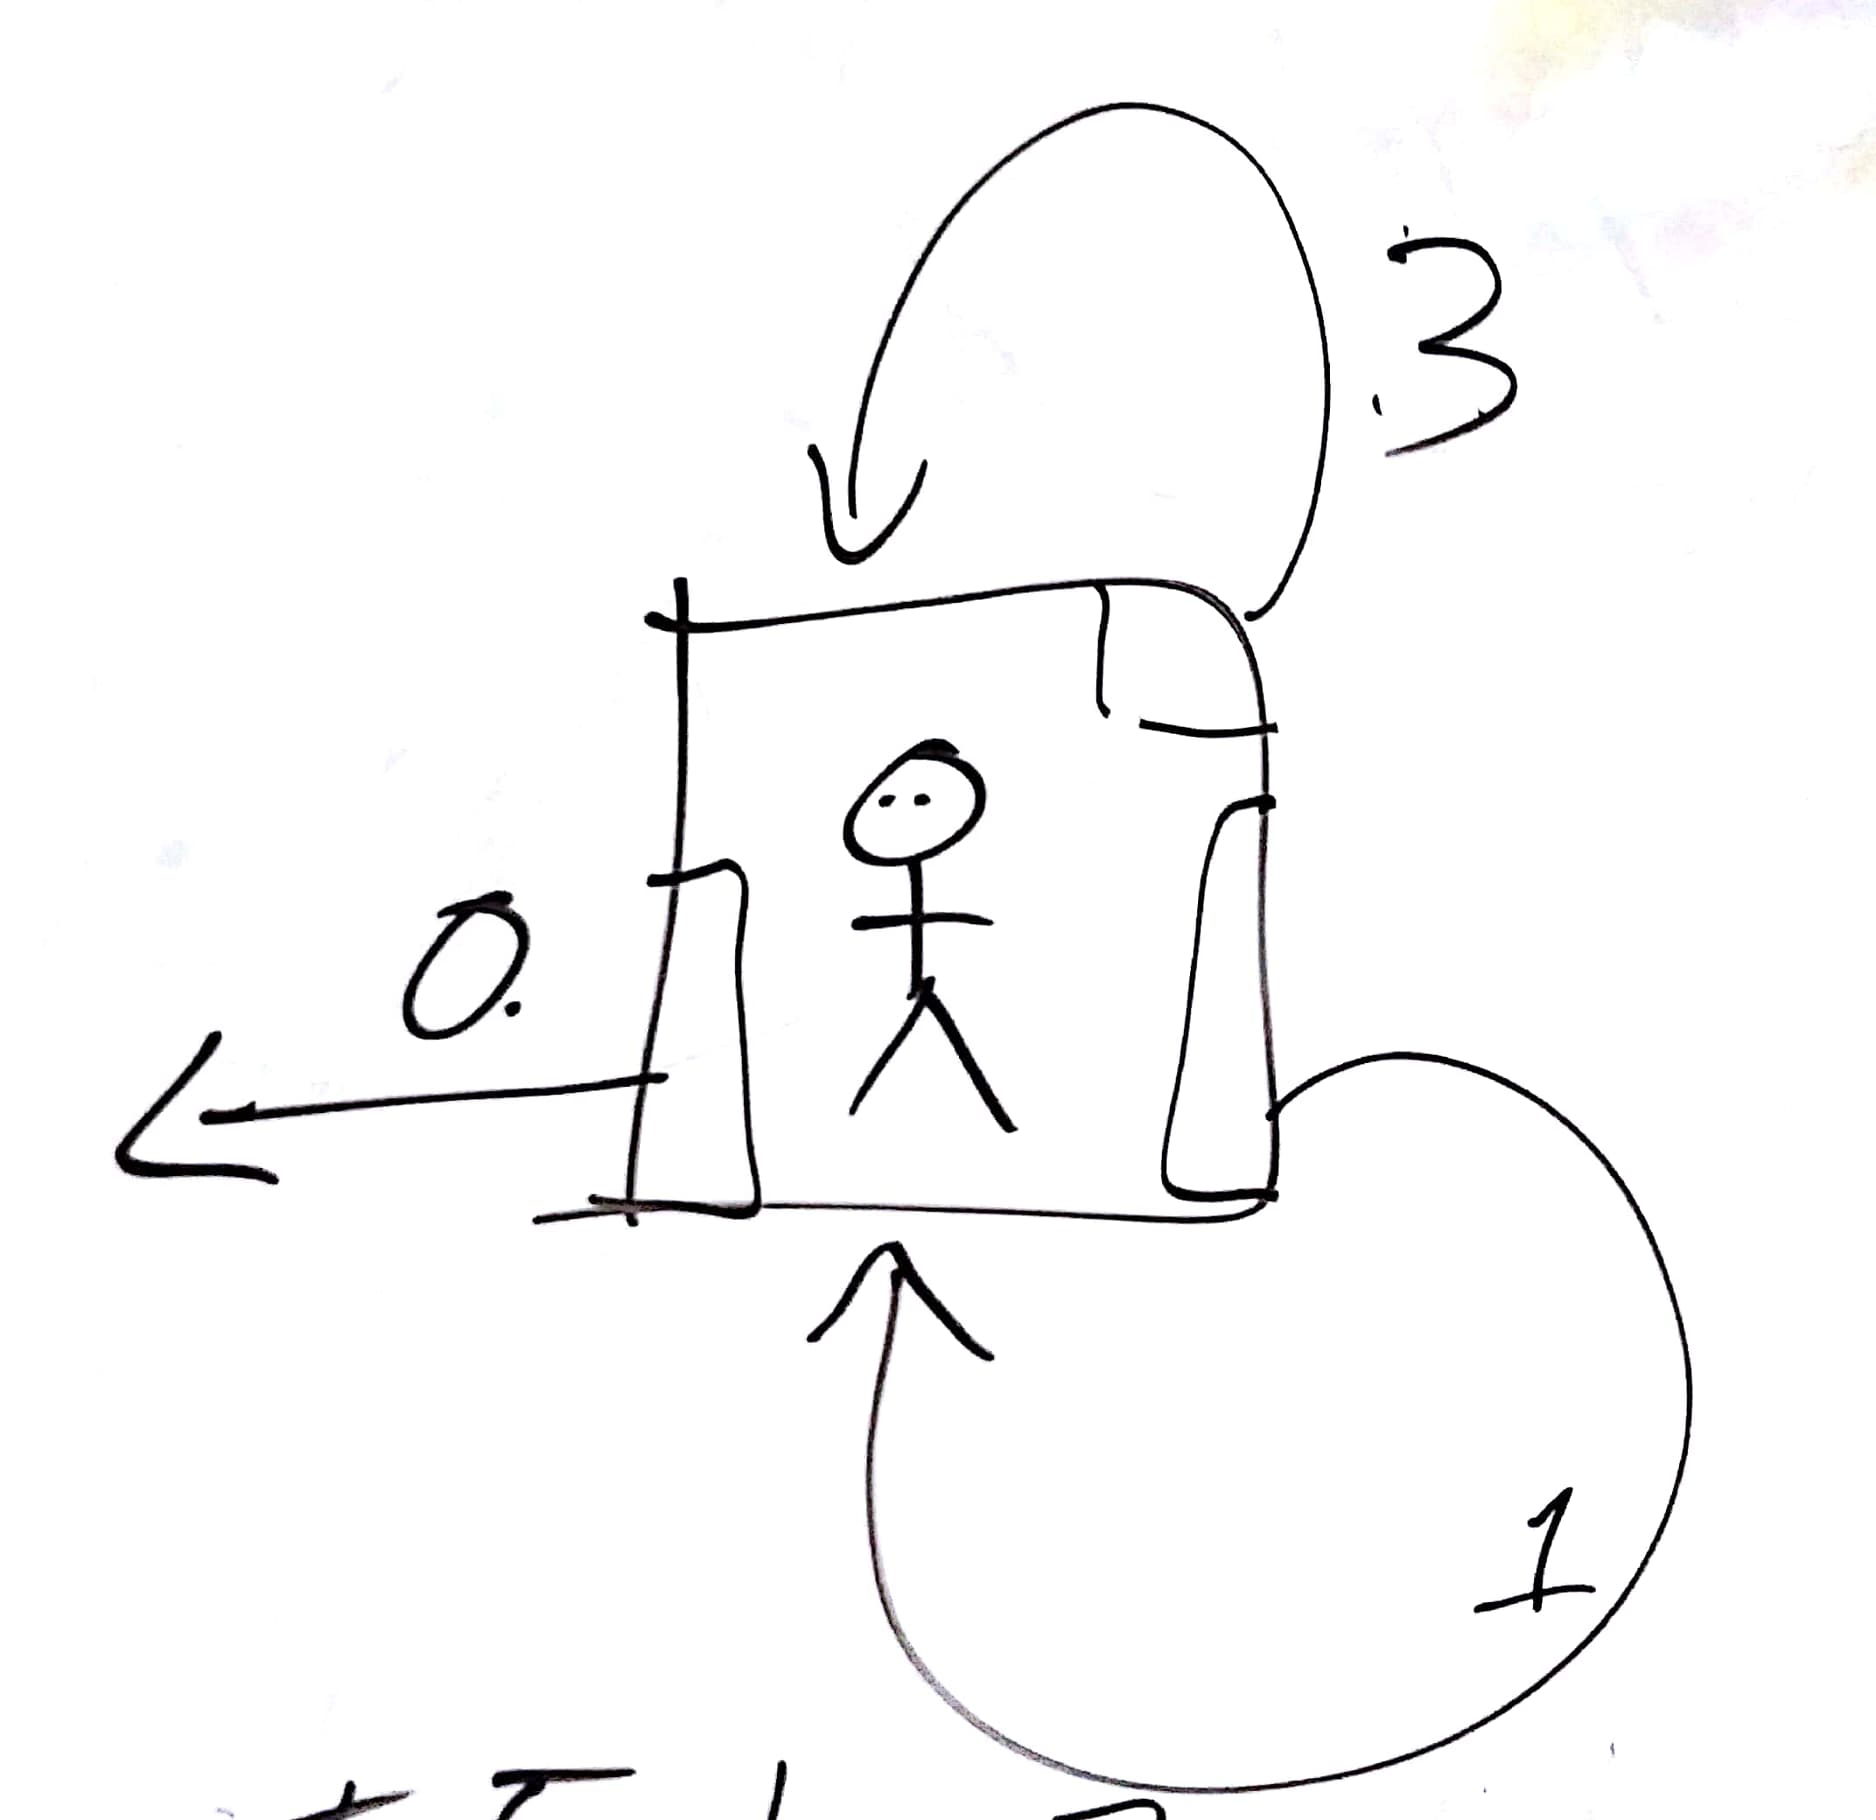
\includegraphics[scale=0.09]{sujeto.jpg}   
        \end{center}\vspace{.1cm}

        $E(X)=(E[X]+1)E[X|X=1]+(E[X]+3)E[X|X=2]$\vspace{.1cm} 
        
        pero $E[X|X=1]=E[X|X=2]=E[X|X=3]=\frac{1}{3}$\vspace{.1cm}

        $\Rightarrow E[x]=\frac{E[X]}{3}+\frac{1}{3}+\frac{E[X]}{3}+\frac{3}{3}=\frac{2E[X]}{3}+\frac{4}{3}$\vspace{.1cm}

        $\Rightarrow \frac{E[X]}{3}=\frac{3}{4} \Rightarrow E[X]=4$\vspace{.3cm}

        11. Sea $f(x) = \left \{ 
            \begin{matrix}
                6x(1-x)$\hspace{1cm} si $0 < x < 1 \\ $
                $0$ \hspace{1cm} $e.o.c$
            $\end{matrix}
        \right .$\vspace{.1cm}
        
        a) Calcula la media y la varianza de la variable aleatoria $X$ 
        con distribución $f(x)$\vspace{.1cm}

        \framebox{Solución}\vspace{.1cm}

        $Media=E(x)=\displaystyle\int_{0}^{1}x(6x-6x^2)dx = 
        \int_{0}^{1}6x^2dx-\int_{0}^{1}6x^3dx = \left. \frac{6x^3}{3} \right |_{0}^{1}
         - \left. \frac{6x^4}{4} \right |_{0}^{1} = 2 - \frac{3}{2} = \frac{1}{2}$\vspace{.1cm}

        b) Encuentra el n-ésimo momento de la variable aleatoria $X$ 
        con distribución $f(x)$\vspace{.1cm}

        \framebox{Solución}\vspace{.1cm}

        $Var(x) = E(x^2) - E^2(x)$\vspace{.1cm}

        $E(x^2) = \displaystyle\int_{0}^{1}x^2(6x-6x^2)dx = \int_{0}^{1}(6x^3-6x^4)dx = 
        \left .(\frac{3x^4}{2} - \frac{6x^5}{5})\right |_{0}^{1} 
        = \frac{3}{2} - \frac{6}{5} = \frac{3}{10}$
        \vspace{.1cm}

        $Var(x) = \frac{3}{10} - \frac{1}{4} = \frac{1}{20}$\vspace{.1cm}

        c) Encuentra su función generadora de momentos\vspace{.1cm}

        \framebox{Solución}\vspace{.1cm}

        $M(t) = E(e^{tx}) = \int_{0}^{1}e^{tx}(6x-6x^2)dx 
        = \int_{0}^{1}6xe^{tx}dx - \int_{0}^{1}6x^2e^{tx}dx =
        -6\int_{0}^{1}x^2e^{tx}dx + 6\int_{0}^{1}xe^{tx}dx$
        
        Integrando por partes, tenemos que: \vspace{.1cm}

        $M(t) = \frac{6(e^t(t-2)+t+2)}{t^3}$\vspace{.3cm}

        12. Demuestra o proporciona un contraejemplo: \vspace{.1cm}

        a) $Var(E(X)) = E(X)$\vspace{.1cm}

        \framebox{Solución:}\vspace{.1cm}

        FALSO. \underline{Contraejemplo:}\vspace{.1cm}

        $f(x) = \left \{ 
            \begin{matrix}
                1$\hspace{1cm} si $x = 1 \\ $
                $0$ \hspace{1cm} $e.o.c$
            $\end{matrix}
        \right .$\vspace{.1cm}

        $E[X]= (1)(1)=1$\vspace{.1cm}

        $Var(X)=0\neq 1 = E[x]$\vspace{.1cm}

        $\therefore$ $E[X]\neq Var(E[X])$\vspace{.2cm}
        
        b) $E(Var(X)) = Var(X)$ \vspace{.1cm}

        \framebox{Demostración:}\vspace{.1cm}

        Sea $X$ una variable aleatoria.\vspace{.1cm}

        $c=Var(X)\in \mathbb{R^+}$\vspace{.1cm}

        $E[c]=c$\vspace{.1cm}

        $\therefore$ $E[Var(X)]=Var(V)$\vspace{.3cm}

        13. Encuentra la función generadora de momentos de $X$ y, 
        a partir de ella, calcula la media y la varianza de $X$ 
        \vspace{.3cm}

        a)$f(x) = \left \{ 
            \begin{matrix}
                \frac{1}{2^x}$\hspace{1cm} si $x = 1,2,... \\ $
                $0$ \hspace{1cm} $e.o.c$
            $\end{matrix}
        \right .$\vspace{.1cm}

        b)$f(x) = \left \{ 
                \begin{matrix}
                    e^{-x}$\hspace{1cm} si $x > 0 \\ $
                    $0$ \hspace{1cm} $e.o.c$
                $\end{matrix}
            \right .$\vspace{.3cm}

        14. Una póliza de seguro grupal cubre los reclamos médicos 
        de los empleados de una pequeña empresa. El valor, $V$, de 
        las reclamaciones hechas en un año se describe por 
        $V=100,000$ donde $Y$ es una variable aleatoria con 
        f.d.p $f(y) = \left \{ 
            \begin{matrix}
                k(1-y)^4$\hspace{1cm} si $0 < x < 1 \\ $
                $0$ \hspace{1cm} $e.o.c$
            $\end{matrix}
        \right .$ donde k es una constante. ¿Cuál es la probabilidad 
        de que $V$ exceda $40,000$ dado que $V$ excede $10,000$?
        \vspace{.1cm}

        \framebox{Solución}\vspace{.1cm}

        $k\displaystyle\int_{0}^{1}(1-y)^4 = k\displaystyle\int_0^1(y^4-4y^3+6y^2-4y+1)dy 
        = k \left . \frac{y^5}{5} - y^4 + 2y^3 - 2y^2 + y \right |_0^1 = 
        k (\frac{1}{5} - 1 + 2 - 2 + 1) = k (\frac{1}{5})$, luego: \vspace{.1cm}

        $\frac{k}{5} = 1$\vspace{.1cm}

        $k = 5$\vspace{.3cm}

        15. Una compañía de seguros asegura una gran cantidad de 
        viviendas. Se supone que el valor asegurado $X$ de una 
        vivienda seleccionada al azar, tiene la siguiente f.d.p.\vspace{.1cm}

        $f(x) = \left \{ 
                \begin{matrix}
                    3x^{-4}$\hspace{1cm} si $x > 1 \\ $
                    $0$ \hspace{1cm} $e.o.c$
                $\end{matrix}
            \right .$\vspace{.1cm}
        
            Dada que una casa seleccionada al azar está asegurada 
            por al menos 1.5, ¿Cuál es la probabilidad de que esté 
            asegurado por menos de 2?\vspace{.1cm}

            \framebox{Solución}\vspace{.1cm}

            $\mathbb{P}(-1.5 \leq x < 2) = \int_{1.5}^{2}3x^{-4}dx 
            = 3 (\left .\frac{x^{-3}}{-3})\right |_1.5^2) = 3 (\frac{37}{648}) = \frac{111}{648}
            =0.1712$\vspace{.1cm}
    
            $\therefore 17.12\%$\vspace{.3cm}

        16. La pérdida debida a un incendio en un edificio comercial 
        está modelada por la variable aleatoria $X$ con f.d.p. \vspace{.1cm}

        $f(x) = \left \{ 
                \begin{matrix}
                    0.005(20-x)$\hspace{1cm} si $0 < x < 20 \\ $
                    $0$ \hspace{1cm} $e.o.c$
                $\end{matrix}
            \right .$\vspace{.1cm}

        Dado que una pérdida de incendio excede de 8. ¿Cuál es 
        la probabilidad de que exceda 16?\vspace{.1cm}

        \framebox{Solución}\vspace{.1cm}

        $\mathbb{P}(x>8) = \displaystyle\int_8^{20}(0.005)(20-x)dx = 
        (0.005)(\left . 20x - \frac{x^2}{2} \right |_{8}^{20}) = 
        (20(20) - \frac{20^2}{2}) - (20(8) - \frac{8^2}{2})$\vspace{.1cm} 

        $= 0.005(200 - 128) = 0.005(72) = .36$\vspace{.1cm}

        $\mathbb{P}(x>16) = \displaystyle\int_{16}^{20}(0.005)(20-x)dx = 
        (0.005)(\left . 20x - \frac{x^2}{2} \right |_{16}^{20}) = 
        (20(20) - \frac{20^2}{2}) - (20(16) - \frac{16^2}{2})$ \vspace{.1cm}

        $= 0.04$\vspace{.3cm}

        17. La vida útil de un aparato tiene una distribución 
        continua en el intervalo $(0,40)$ con f.d.p \vspace{.1cm}

        $f(x)=(10+x)^{-2}$\vspace{.1cm}

        Calcula la probabilidad de que la vida útil del aparato sea 
        menor a 6.\vspace{.1cm}

        \framebox{Solución}\vspace{.1cm}

        $\mathbb{P}(x < 6) = \int_{0}^{6}(10+x)^{-2}dx$, 
        Hagamos cambio de variable \vspace{.1cm}

        $u = 10 + x$, y $du = dx$, entonces los limites quedan como $10$ y $16$, entonces \vspace{.1cm}

        $\mathbb{P}(x < 6) = \int_{10}^{16}\frac{1}{u^2}du = \left . (\frac{-1}{u}) \right |_{10}^{16} = \frac{3}{80} $
        \vspace{.3cm}

        18. Sea $X$ variable aleatoria con f.d.p $f(x) = \left \{ 
            \begin{matrix}
                1.4e^{-2x}+0.9e^{-3x}$\hspace{1cm} si $x > 0 \\ $
                $0$ \hspace{1cm} $e.o.c$
            $\end{matrix}
        \right .$: calcula $E(X)$\vspace{.1cm}

        \framebox{Solución}\vspace{.1cm}

        $E(X) = \displaystyle\int_{0}^{\infty}x(1.4e^{-2x}+0.9e^{-3x})dx 
        = \left . e^{-3x}(e^{5x}(.7x-.35)-.3x-.1) \right |_{0}^{\infty} 
        = 0 - 1(1(0-.35)+.1) = \frac{9}{20}$\vspace{.3cm}

        19. Sea $X$ una variable aleatoria continua con f.d.p. 
        $f(x) = \left \{ 
                \begin{matrix}
                    \frac{1}{9}x(4-x)$\hspace{1cm} si $0 < x < 3 \\ $
                    $0$ \hspace{1cm} $e.o.c$
                $\end{matrix}
            \right .$: ¿Cuál es la moda de $X$?\vspace{.1cm}

        \framebox{Solución}\vspace{.1cm}

        Derivamos la funcion de densidad de probabilidad, tenemos que:\vspace{.1cm}

        $f'(x) = \frac{4}{9} - \frac{2x}{9}$, igualamos a cero para obtener el máximo\vspace{.1cm}

        $\frac{4}{9} - \frac{2x}{9} = 0$\vspace{.1cm}

        $\frac{2x}{9} = \frac{4}{9}$\vspace{.1cm}

        $x = 2$\vspace{.1cm}

        Evaluamos antes y después en la original para ver que sea máximo. \vspace{.1cm}

        $f(1) = \frac{1}{9}(3) = \frac{3}{9}$\vspace{.1cm}

        $f(4) = \frac{4}{9}(0) = 0$\vspace{.1cm}

        $\therefore$ Es máximo

        20. En la siguiente tabla se muestra una distribución de 
        probabilidad de los tamaños de reclamación para una 
        póliza de seguros de autos. \vspace{.1cm}
        
        \begin{center}
            \begin{tabular}{| c | c | c | c | c | c | c | c |}
                \hline
                Tamaño de la reclamación & 20 & 30 & 40 & 50 & 60 & 70 & 80\\ \hline
                Probabilidad & .15 & .1 & .05 & .2 & .1 & .1 & .3\\ \hline
            \end{tabular} \vspace{.1cm}    
        \end{center}

        ¿Qué porcentaje de las reclamaciones se encuentran dentro 
        de una desviación estándar del tamaño promedio de la 
        reclamación?\vspace{.1cm}

        \framebox{Solución}\vspace{.1cm}

        Desviación estándar: $\sqrt{\frac{\displaystyle\sum(|x-prom(x)|)}{n}}$\vspace{.1cm}

        $prom(x) = 50$\vspace{.1cm}

        $|x_{i}-prom(x_{i})|^2 = |20-50|^2 + |30-50|^2 + |40-50|^2 
        + |50-50|^2 + |60-50|^2 + |70-50|^2 + |80-50|^2 = 4600$\vspace{.1cm}

        $sqrt{\frac{4600}{7}} = 25.634$\vspace{.1cm}

        Coeficiente de variacion: $\frac{\Sigma}{|prom(x)|}*100$\vspace{.1cm}

        Coeficiente de variación $= 51.2\%$

        21. Un actuario determina que el tamaño de la reclamación 
        para una determinada clase de accidente es una variable 
        aleatoria $X$, con función generadora de momentos 
        $M_x(t)=\frac{1}{(1-2500t)^4}$; determina la desviación 
        estándar del tamaño de la reclamación para esta clase de 
        accidentes.\vspace{.1cm}

        \framebox{Solución}\vspace{.1cm}

        $M'_x(t)=\frac{-4(\frac{d}{dt}(1-2500t))}{(1-2500t)^5} 
        = \frac{-4}{(1-2500t)^5}-2500\frac{d}{dt} = \frac{10000}{(1-2500t)^5}$, 
        ahora evaluemos en $t=0$ \vspace{.1cm}

        $M'_x(t) = \frac{10000}{1^5}= 10000$\vspace{.1cm}

        Ahora calculemos el segundo momento\vspace{.1cm}

        $M''_x(t) = 10000 \frac{d}{dt}(\frac{1}{(1-2500t)^5}) = 
        10000 (\frac{-5\frac{d}{dt}(1-2500t)}{(1-2500t)^6}) = 
        \frac{-50000(\frac{d}{dt}(1-2500t))}{(1-2500t)^6} = 
        \frac{125000000}{(1-2500t)^6} = 5000$ \vspace{.1cm}

        Ahora calculemos la varianza de x: \vspace{.1cm}

        $Var(x) = E(x^2) - E^2(x) = 125000000 - 10000^2 = 25000000$\vspace{.1cm}

        Y tenemos que la desviación estándar es: $\displaystyle\sqrt(Var(x)) 
        = \displaystyle\sqrt(25000000) = 5000$\vspace{.3cm}

        22. La función generadora de momentos de la variable 
        aleatoria $X$ está dada por $M_x(t)=\frac{1}{(1+t)}$, 
        encuentra el tercer momento de $X$ sobre el punto $x=2$
        \vspace{.1cm}

        \framebox{Solución}\vspace{.1cm}

        $\frac{d}{dx}M_x(t)=-\frac{1}{(1+t)^2} \Rightarrow \frac{d}{dx}M_x(0)=-1=E(X)$\vspace{.1cm}

        $\frac{d^2}{dx^2}M_x(t)=\frac{2}{(1+t)^3} \Rightarrow \frac{d^2}{dx^2}M_x(0)=2=E(X^2)$\vspace{.1cm}

        $\frac{d^3}{dx^3}M_x(t)=-\frac{6}{(1+t)^4} \Rightarrow \frac{d^3}{dx^3}M_x(0)=-6 = E(X^3)$\vspace{.1cm}

        Tenemos que calcular $E[(X-c)^3]$\vspace{.1cm}

        $E[(X-c)^3]=E[X^3-3X^2c+3Xc^2-c^3]=E(X^3)-3E(X^2)c+3E(X)c^2-c^3$\vspace{.1cm}

        $E[(X-c)^3]=-6-6c+c^2-c^3$

        23. Una variable aleatoria tiene la siguiente función de 
        distribución.\vspace{.1cm}

        $F(x) = \left \{ 
                \begin{matrix}
                    0$\hspace{1cm} para $x < 1 \\ $
                    $\frac{x^2-2x+2}{2}$ \hspace{1cm} $1 \leq x < 2 \\$
                    $1$ \hspace{1cm} para $x \geq 2$
                $\end{matrix}
            \right .$\vspace{.1cm}

        Encuentra la varianza de $X$.\vspace{.3cm}

        24. El monto de la pérdida $X$, para una póliza de seguro 
        médico tiene una función de distribución\vspace{.1cm}

        $F(x) = \left \{ 
                \begin{matrix}
                    0$\hspace{1cm} para $x < 0 \\ $
                    $\frac{1}{9}(2x^2-\frac{x^3}{3})$ \hspace{1cm} para $0 \leq x \leq 3 \\$
                    $1$ \hspace{1cm} para $x > 3$
                $\end{matrix}
            \right .$\vspace{.1cm}

        Calcula la moda de la distribución.\vspace{.1cm}

        \framebox{Solución:}\vspace{.1cm}

        Para calcular la moda de la distribución se tiene que calcular $f.d.p.$ entonces $\frac{d}{dx}(F_x(x))=f_x(x)$\vspace{.1cm}

        $\frac{d}{dx}(\frac{2x^2}{9}-\frac{x^3}{27})=\frac{4x}{9}-\frac{x^2}{9}$\vspace{.1cm}

        $\Rightarrow x(\frac{4}{9}-\frac{x}{9}) \Rightarrow x = 0 \Rightarrow \frac{4}{9}= \frac{x}{9} \Rightarrow x = 4$\vspace{.2cm}

        Entonces, $x=0$ ó $x=4$. $\therefore$ la moda de la función de distribución es 4.\vspace{.3cm}

        25. La variable aleatoria $X$ tiene f.d.p. $f(x)=ce^{-|x|}$ para $-\infty<x<\infty$. 
        Encuentra la varianza de $X$.

        \begin{center}
            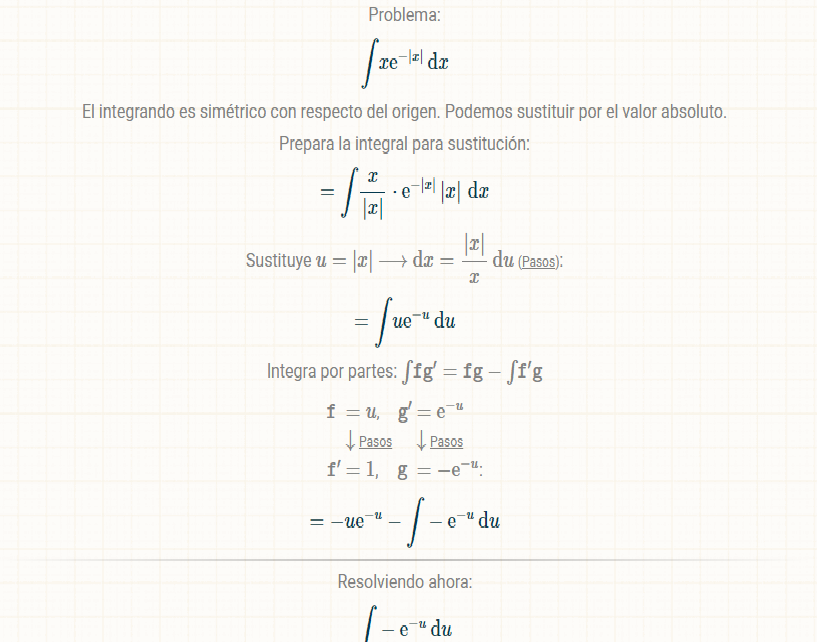
\includegraphics[scale=0.4]{proba2.png}   
        \end{center}

        \begin{center}
            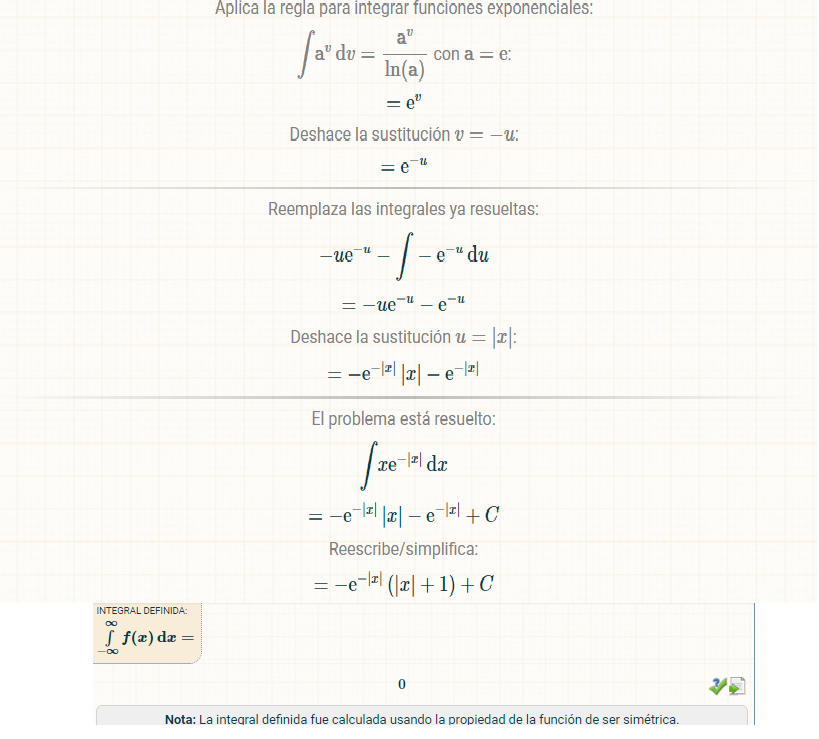
\includegraphics[scale=0.4]{proba3.png}
        \end{center}
    \end{document}